\begin{figure}[ht]
    \centering
    \begin{subfigure}{.49\textwidth}
        \centering
        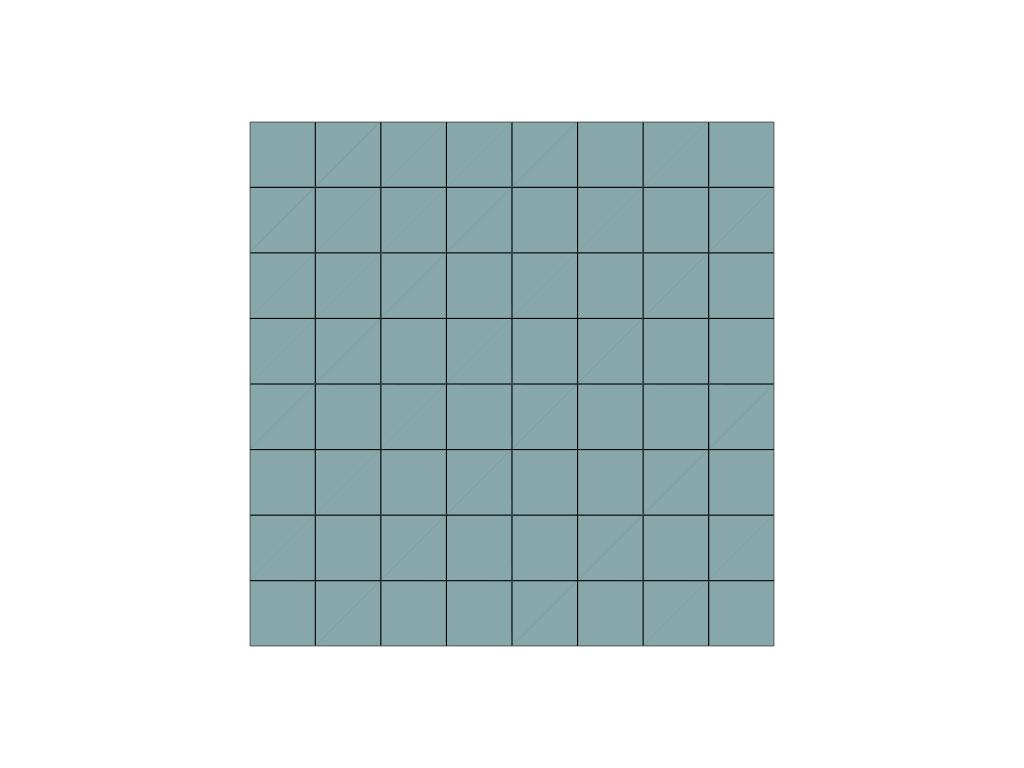
\includegraphics[width=\textwidth]{Afsnit/Application/figurer/screenshot_1.jpeg}
        \caption{Domain partitioned into triangles}~\label{fig:FEM_plot_domain}
      \end{subfigure}
    \begin{subfigure}{.49\textwidth}
        \centering
        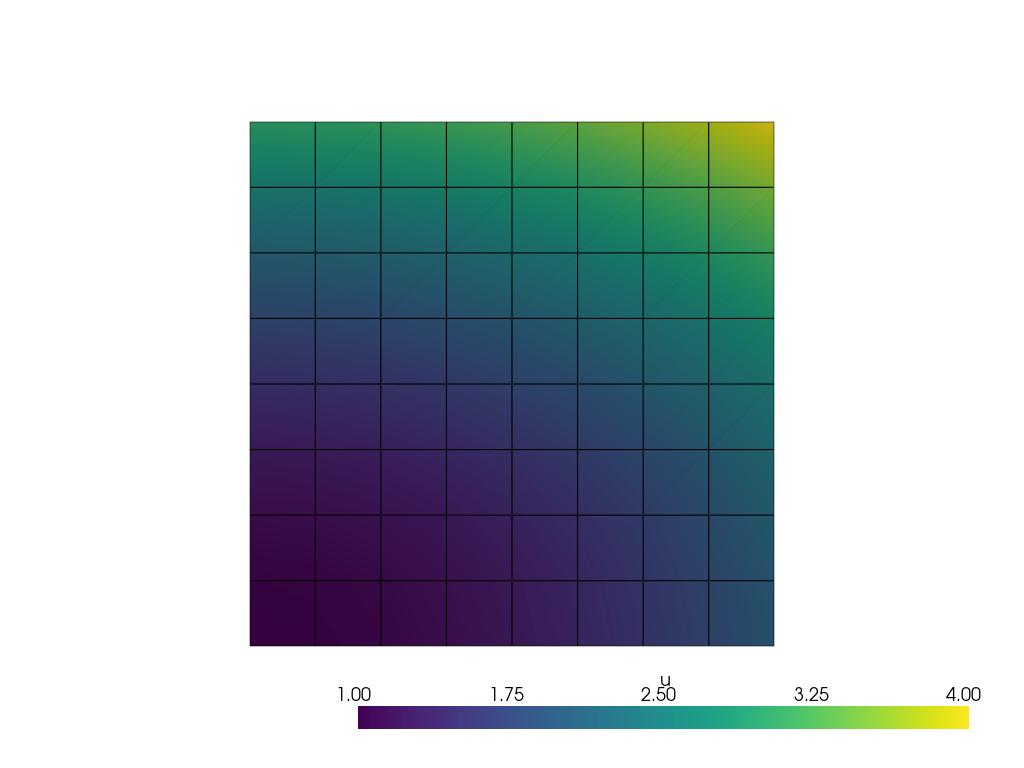
\includegraphics[width=\textwidth]{Afsnit/Application/figurer/screenshot_2.jpeg}
        \caption{Domain colored in accordance to the warping scalar obtained by the solution $u_h$ ranging from $-1.06$ to $4.40$}~\label{fig:FEM_plot_warped_domain}
    \end{subfigure}
    \begin{subfigure}{.49\textwidth}
        \centering
        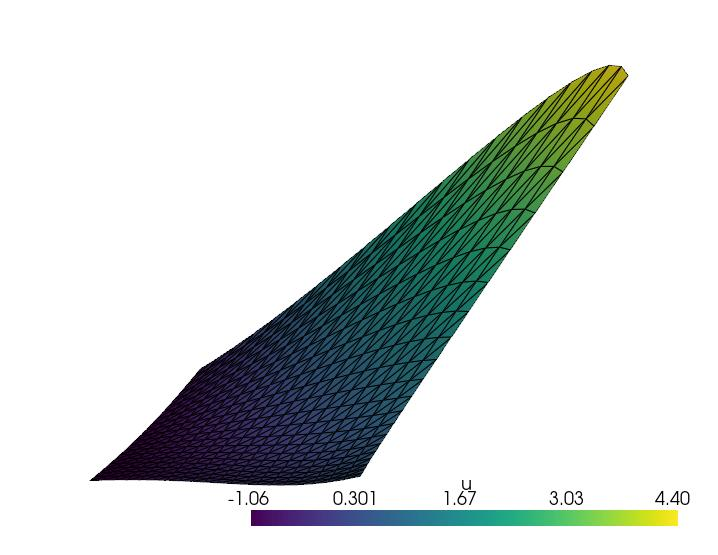
\includegraphics[width=\textwidth]{Afsnit/Application/figurer/screenshot_3.jpeg}
        \caption{The same domain warped with respect to the scalar value, ranging from $-1.06$ to $4.40$}~\label{fig:FEM_plot_3D}
    \end{subfigure}
    \caption{Plots of the domain}~\label{fig:FEM_plots}
\end{figure}

As discussed earlier the first step in approximating the solution to a PDE is to establish a fitting domain. In our example we have chosen a square ranging from $(-1,-1)$ to $(1,1)$.
We have chosen to partition into triangles, as can be seen
in Figure~\ref{fig:FEM_plot_domain}. 
These triangles are of equal size making the domain regular.
After the domain is partitioned and we have estimated the solution,
we can plot the solution over the domain to obtain Figure~\refeq{fig:FEM_plot_warped_domain} 
where each cell is coloured in accordance to the value in the given point.
We can then warp the domain to give a clear look on what exactly our solution looks like in 3D, 
which is shown in Figure~\refeq{fig:FEM_plot_3D}.
%, 
%where it is also obvious what the visual meaning of a boundary condition is, 
%since it is clear the boundary follows the specificied function $1 + x_0^2 + 2x_1^2$.